\documentclass[border=10pt]{standalone}
\usepackage{pgfplots}
\pgfplotsset{compat=1.18}
\begin{document}
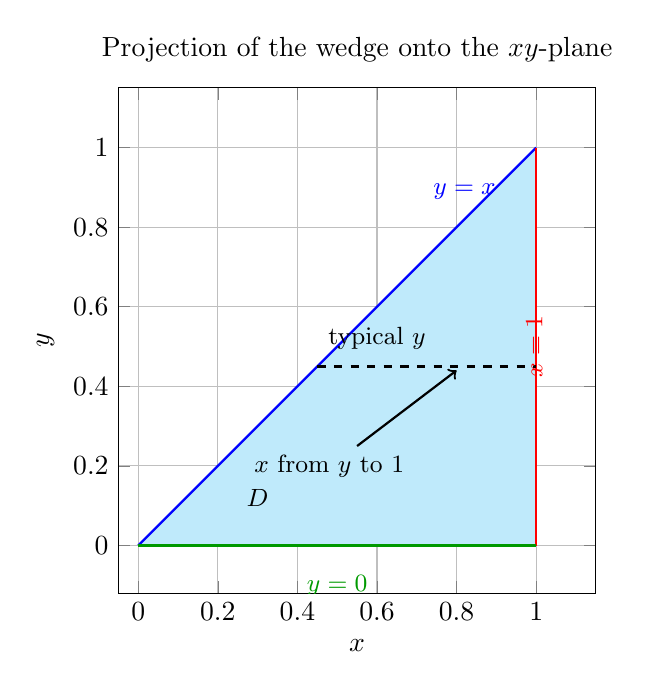
\begin{tikzpicture}
\begin{axis}[
    width=9cm, height=8cm,
    axis equal image,
    xmin=-0.05, xmax=1.15, ymin=-0.12, ymax=1.15,
    xlabel={$x$}, ylabel={$y$},
    title={Projection of the wedge onto the $xy$-plane},
    grid=both,
]
% shaded triangular region D
\addplot[fill=cyan!25, draw=none] coordinates {(0,0) (1,1) (1,0)} \closedcycle;
% boundary y = x
\addplot[blue, thick, domain=0:1] {x};
% boundary x = 1
\addplot[red, thick] coordinates {(1,0) (1,1)};
% boundary y = 0
\addplot[green!60!black, thick] coordinates {(0,0) (1,0)};
% typical horizontal slice
\addplot[black, dashed, thick] coordinates {(0.45,0.45) (1,0.45)};
% labels
\node[text=blue, font=\small] at (axis cs:0.82,0.89) {$y=x$};
\node[text=red, font=\small, rotate=90, anchor=south] at (axis cs:1.04,0.5) {$x=1$};
\node[text=green!60!black, font=\small, anchor=north] at (axis cs:0.5,-0.05) {$y=0$};
\node[font=\small] at (axis cs:0.30,0.12) {$D$};
\node[font=\small] at (axis cs:0.60,0.52) {typical $y$};
\draw[->, thick] (axis cs:0.55,0.25) -- (axis cs:0.80,0.44);
\node[font=\small] at (axis cs:0.48,0.20) {$x$ from $y$ to $1$};
\end{axis}
\end{tikzpicture}
\end{document}